\documentclass[12pt]{article}\usepackage[]{graphicx}\usepackage[]{color}
%% maxwidth is the original width if it is less than linewidth
%% otherwise use linewidth (to make sure the graphics do not exceed the margin)
\makeatletter
\def\maxwidth{ %
  \ifdim\Gin@nat@width>\linewidth
    \linewidth
  \else
    \Gin@nat@width
  \fi
}
\makeatother

\definecolor{fgcolor}{rgb}{0.345, 0.345, 0.345}
\newcommand{\hlnum}[1]{\textcolor[rgb]{0.686,0.059,0.569}{#1}}%
\newcommand{\hlstr}[1]{\textcolor[rgb]{0.192,0.494,0.8}{#1}}%
\newcommand{\hlcom}[1]{\textcolor[rgb]{0.678,0.584,0.686}{\textit{#1}}}%
\newcommand{\hlopt}[1]{\textcolor[rgb]{0,0,0}{#1}}%
\newcommand{\hlstd}[1]{\textcolor[rgb]{0.345,0.345,0.345}{#1}}%
\newcommand{\hlkwa}[1]{\textcolor[rgb]{0.161,0.373,0.58}{\textbf{#1}}}%
\newcommand{\hlkwb}[1]{\textcolor[rgb]{0.69,0.353,0.396}{#1}}%
\newcommand{\hlkwc}[1]{\textcolor[rgb]{0.333,0.667,0.333}{#1}}%
\newcommand{\hlkwd}[1]{\textcolor[rgb]{0.737,0.353,0.396}{\textbf{#1}}}%

\usepackage{framed}
\makeatletter
\newenvironment{kframe}{%
 \def\at@end@of@kframe{}%
 \ifinner\ifhmode%
  \def\at@end@of@kframe{\end{minipage}}%
  \begin{minipage}{\columnwidth}%
 \fi\fi%
 \def\FrameCommand##1{\hskip\@totalleftmargin \hskip-\fboxsep
 \colorbox{shadecolor}{##1}\hskip-\fboxsep
     % There is no \\@totalrightmargin, so:
     \hskip-\linewidth \hskip-\@totalleftmargin \hskip\columnwidth}%
 \MakeFramed {\advance\hsize-\width
   \@totalleftmargin\z@ \linewidth\hsize
   \@setminipage}}%
 {\par\unskip\endMakeFramed%
 \at@end@of@kframe}
\makeatother

\definecolor{shadecolor}{rgb}{.97, .97, .97}
\definecolor{messagecolor}{rgb}{0, 0, 0}
\definecolor{warningcolor}{rgb}{1, 0, 1}
\definecolor{errorcolor}{rgb}{1, 0, 0}
\newenvironment{knitrout}{}{} % an empty environment to be redefined in TeX

\usepackage{alltt}

\usepackage[margin=0.75in]{geometry}


\title{Rnw Files}
\author{Gaston Sanchez}
\date{\today}
\IfFileExists{upquote.sty}{\usepackage{upquote}}{}
\begin{document}
\maketitle

\noindent This is a simple example on how to use Rnw files. At one time, the phrase, You've got mail, was a welcomed, even exciting notification. Our inboxes were usually empty, so we eagerly anticipated the arrival of \dots Read More.

Here's a table displayed with the R package \texttt{"xtable"}

% latex table generated in R 3.2.3 by xtable 1.8-2 package
% Tue Mar  8 17:09:30 2016
\begin{table}[ht]
\centering
\begin{tabular}{rllll}
  \hline
 &  Sepal.Length &  Sepal.Width &  Petal.Length &  Petal.Width \\ 
  \hline
1 & Min.   :4.300   & Min.   :2.000   & Min.   :1.000   & Min.   :0.100   \\ 
  2 & 1st Qu.:5.100   & 1st Qu.:2.800   & 1st Qu.:1.600   & 1st Qu.:0.300   \\ 
  3 & Median :5.800   & Median :3.000   & Median :4.350   & Median :1.300   \\ 
  4 & Mean   :5.843   & Mean   :3.057   & Mean   :3.758   & Mean   :1.199   \\ 
  5 & 3rd Qu.:6.400   & 3rd Qu.:3.300   & 3rd Qu.:5.100   & 3rd Qu.:1.800   \\ 
  6 & Max.   :7.900   & Max.   :4.400   & Max.   :6.900   & Max.   :2.500   \\ 
   \hline
\end{tabular}
\end{table}


Example of a code chunk:
\begin{knitrout}
\definecolor{shadecolor}{rgb}{0.969, 0.969, 0.969}\color{fgcolor}\begin{kframe}
\begin{alltt}
\hlcom{# two vectors}
\hlstd{x} \hlkwb{<-} \hlnum{1}\hlopt{:}\hlnum{10}
\hlstd{y} \hlkwb{<-} \hlstd{x}\hlopt{*}\hlnum{2} \hlopt{+} \hlnum{5}
\end{alltt}
\end{kframe}
\end{knitrout}

Here's an example of inline code chunk using \texttt{\textbackslash Sexpr\{\}}: the mean value of \texttt{y} is 16, the median of \texttt{y} is 16, and its length is 10


\section{Plot}

More lines
\begin{knitrout}
\definecolor{shadecolor}{rgb}{0.969, 0.969, 0.969}\color{fgcolor}\begin{kframe}
\begin{alltt}
\hlkwd{plot}\hlstd{(x, y)}
\end{alltt}
\end{kframe}
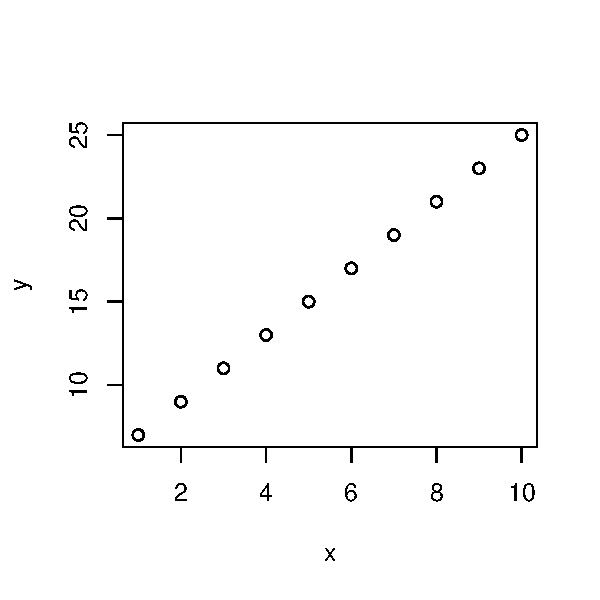
\includegraphics[width=\maxwidth]{figure/plot1-1} 

\end{knitrout}

\end{document}
